\newpage
~
\newpage
\chapter{Introducción}

\section{Contexto}

En la era digital actual, la generación de contenido multimedia personal ha alcanzado niveles sin precedentes. La aparición de teléfonos inteligentes equipados con cámaras de alta resolución ha convertido a cada individuo en un creador de contenido, documentando su vida a través de miles de fotografías y vídeos. Este vasto volumen de datos requiere soluciones de almacenamiento robustas, accesibles y, sobre todo, duraderas.

En respuesta a esta demanda, han surgido gigantes tecnológicos que ofrecen servicios de almacenamiento en la nube, como Google Photos, Apple iCloud y Amazon Photos. Estas plataformas proporcionan una comodidad innegable: sincronización automática entre dispositivos, copias de seguridad sin esfuerzo y potentes herramientas de organización basadas en \gls{ia}. Sin embargo, este modelo de servicio centralizado presenta una serie de inconvenientes significativos que a menudo pasan desapercibidos para el usuario promedio.

El primer y más crítico es la \textbf{privacidad}. Al subir recuerdos personales a servidores de terceros, se cede una parte considerable del control sobre los datos. Estos archivos pueden ser analizados para fines publicitarios, sujetos a políticas de servicio que cambian unilateralmente y, en última instancia, vulnerables a brechas de seguridad fuera de nuestro control. Este factor lleva al usuario a depositar su confianza en estas corporaciones, a menudo de manera injustificada.

El segundo factor es el \textbf{coste económico}. La mayoría de estos servicios operan bajo un modelo \textit{freemium}, ofreciendo un nivel de almacenamiento gratuito inicial que, para la mayoría de los usuarios, resulta insuficiente a medio plazo. Una vez superado este umbral, se ven obligados a suscribirse a planes de pago mensuales o anuales, generando una dependencia económica continua para poder seguir almacenando sus propios recuerdos.

En tercer lugar, existe el problema del \textbf{vendor lock-in} o dependencia del proveedor. Migrar una biblioteca de miles de fotos y vídeos de un servicio a otro es un proceso a menudo complejo y tedioso. Las herramientas de exportación pueden ser limitadas, y los metadatos valiosos (como álbumes, etiquetas o datos de reconocimiento facial) rara vez son transferibles, lo que atrapa al usuario en un ecosistema cerrado.

Frente a este panorama, emerge con fuerza el concepto de \textbf{autoalojamiento (self-hosting)}. Esta filosofía defiende devolver al usuario el control total sobre sus datos, alojando los servicios en hardware propio, como un ordenador personal, un servidor doméstico o un NAS (Network Attached Storage). El movimiento del software de código abierto (\acrshort{foss}) ha sido un pilar fundamental para atacar este problema, proveyendo alternativas potentes y transparentes a las soluciones propietarias. Proyectos como Immich, PhotoPrism o Ente, analizados en detalle en el capítulo de \hyperref[sec:estado_del_arte]{Estado del Arte}, demuestran la viabilidad y el creciente interés en soluciones de gestión multimedia que priorizan la soberanía digital del usuario.

Este proyecto se inscribe en esta última tendencia. Busca ofrecer una solución integral que no solo resuelva el problema práctico del almacenamiento limitado, sino que también aborde las preocupaciones fundamentales de privacidad, coste y control.
\section{Motivación}

La inspiración de este proyecto surgió de una situación cotidiana. Durante un periodo vacacional, un familiar cercano expresó su frustración al haberse quedado sin espacio de almacenamiento en Google Photos. La solución inmediata que proponía el servicio era, previsiblemente, contratar una suscripción de pago. Este escenario, aparentemente trivial, destapó una problemática mucho más profunda: la de usuarios no técnicos que, por desconocimiento de alternativas, se ven obligados a seguir un modelo de dependencia económica y de cesión de datos sin ser plenamente conscientes de las implicaciones.

La necesidad inmediata era práctica: crear un sistema sencillo que permitiera transferir automáticamente las fotos desde un teléfono móvil a un portátil antiguo disponible en el hogar, utilizando la red WiFi local. Sin embargo, esta idea inicial evolucionó rápidamente hacia una motivación más ambiciosa. No se trataba solo de solucionar un problema puntual, sino de abordar la raíz del mismo: la falta de sistemas accesibles que empoderen a los usuarios para gestionar su propia información.

Desde una perspectiva técnica, el proyecto representa un desafío estimulante. ¿Es posible construir una solución que iguale o supere la experiencia de usuario de los servicios comerciales, pero utilizando tecnologías de código abierto y un modelo descentralizado? Esta pregunta impulsa la exploración de sistemas modernos y de alto rendimiento.
Más allá del reto tecnológico, existe una fuerte motivación filosófica alineada con los principios del software libre. La idea de crear un proyecto \acrshort{foss} desde cero, con una arquitectura clara y una documentación exhaustiva, tiene como fin no solo ofrecer un sistema útil, sino también construir una comunidad a su alrededor. Se busca que otros desarrolladores puedan entender, utilizar y, lo más importante, contribuir al proyecto, fomentando un ecosistema colaborativo que garantice su sostenibilidad y evolución a largo plazo.

Finalmente, este Trabajo de Fin de Grado es, en sí mismo, un motor de aprendizaje. La realización del proyecto implica sumergirse en disciplinas clave de la ingeniería de software: desde el diseño de arquitecturas de sistemas distribuidos y el desarrollo de aplicaciones móviles nativas, hasta la implementación de protocolos de seguridad robustos y la planificación de estrategias de respaldo y recuperación de datos. En la siguiente sección se describen el objetivo general y objetivos específicos de este trabajo, los cuales intentan también resaltar la oportunidad para adquirir conocimientos prácticos y enfrentarse a problemas reales, consolidando la formación académica y preparándose para los desafíos del mundo profesional. En definitiva, la motivación es doble: resolver una necesidad real y tangible para los usuarios y, al mismo tiempo, crecer como ingeniero de software a través de la construcción de una solución completa, moderna y significativa.

\section{Objetivos}
\label{sec:objetivos}
% En infinitivo y concisos. Siguiendo las siglas SMART (Specific, Measurable, Achievable, Relevant, Time-bound).
% Mejor tener objetivos generales y después específicos.

\textbf{Objetivo general}

Desarrollar una solución multiplataforma, multiusuario y open-source para la compartición de archivos multimedia. El sistema permitirá a los usuarios almacenar, sincronizar y gestionar sus fotos y vídeos de manera segura y eficiente, utilizando sus propios dispositivos como servidores de almacenamiento. La solución incluirá un cliente ligero para dispositivos móviles y un servidor robusto, ambos diseñados para facilitar la experiencia del usuario, garantizar la privacidad de los datos.

Para ayudar a alcanzar este objetivo general se describen los siguientes objetivos específicos que se considerarán durante el desarrollo del proyecto:

\textbf{Objetivos específicos}

\begin{itemize}
    \item \textbf{OE1: Análisis, diseño e implementación del sistema} \\
    Analizar, diseñar e implementar un sistema para el almacenamiento y sincronización de archivos multimedia, seleccionando los estilos y patrones arquitectónicos más adecuados (como Cliente/Servidor, Modelo-Vista-Controlador, etc.), e incorporando funcionalidades para la gestión y protección de los archivos mediante la gestión de usuarios y permisos.

    \item \textbf{OE2: Desarrollo del cliente y servidor de sincronización} \\
    Implementar tanto el cliente como el servidor encargados de la sincronización automática de archivos multimedia entre dispositivos, asegurando la compatibilidad multiplataforma y la facilidad de despliegue en diferentes entornos.
    Tanto el cliente como el servidor tendrán que ser lo más eficientes posibles, para que puedan ser instalados en la mayoría de los equipos aunque tengan ciertas limitaciones en cuanto a recursos..

    \item \textbf{OE3: Gestión de usuarios, permisos y seguridad} \\
    Desarrollar un sistema robusto de gestión de usuarios y permisos, incluyendo mecanismos de autenticación, autorización y cifrado de archivos, con el objetivo de garantizar la seguridad y privacidad de los datos almacenados y compartidos.

    \item \textbf{OE4: Publicación y documentación del proyecto} \\
    Publicar el código fuente del proyecto bajo una licencia open-source, asegurando la documentación exhaustiva de todos los componentes y facilitando la comprensión, uso y mantenimiento por parte de la comunidad.

    \item \textbf{OE5: Escalabilidad y mantenimiento} \\
    Diseñar el sistema con una arquitectura desacoplada que permita la escalabilidad horizontal y el mantenimiento sencillo, utilizando tecnologías y soluciones que favorezcan la extensibilidad del sistema.

    \item \textbf{OE6: Copias de seguridad y recuperación} \\
    Implementar mecanismos que permitan la realización de copias de seguridad y la recuperación sencilla de los archivos multimedia, garantizando la integridad y disponibilidad de los datos.

    \item \textbf{OE7: Desarrollo de aplicaciones móviles nativas} \\
    Desarrollar aplicaciones móviles nativas para las plataformas más utilizadas, priorizando el rendimiento, la experiencia de usuario y la facilidad de uso mediante interfaces intuitivas y optimizadas.
\end{itemize}


\section{Planificación}
El desarrollo de este proyecto se separa en varias fases:
\begin{itemize}
    \item \textbf{Fase de análisis del estado del arte y tecnologías disponibles:} Durante esta fase se investiga y analiza el estado del arte de las tecnologías disponibles para el desarrollo del proyecto. Se realiza un estudio de las tecnologías más adecuadas para el desarrollo del cliente y servidor.
    \item \textbf{Fase de especificación de requisitos:} Durante esta fase se realiza el análisis de requisitos y se define la arquitectura del sistema, así como los estilos y patrones arquitectónicos a utilizar. Se definen los requisitos, se elabora un prototipo inicial del sistema y se decide qué tecnologías se van a utilizar para el desarrollo del cliente y servidor.
    \item \textbf{Estudio de las tecnologías seleccionadas:} En esta fase se estudian las tecnologías seleccionadas en el Sprint 0 para el desarrollo del cliente y servidor, para familiarizarse con ellas y poder utilizarlas de manera eficiente en el desarrollo del proyecto. Se comprobará la viabilidad de las tecnologías seleccionadas y se realizarán pruebas iniciales para asegurar que se ajustan a las necesidades del proyecto.
    \item \textbf{Desarrollo del del sistema:} Esta fase aborda el diseño general del sistema y el desarrollo del cliente y el servidor, siguiendo la arquitectura y los patrones arquitectónicos definidos en la fase de especificación de requisitos. Esta fase se dividirá en varias etapas, las cuales se especificarán en su apartado correspondiente.
\end{itemize}

A continuación se muestra el diagrama de Gantt con la planificación del proyecto:
\begin{figure}[H]
    \begin{center}
        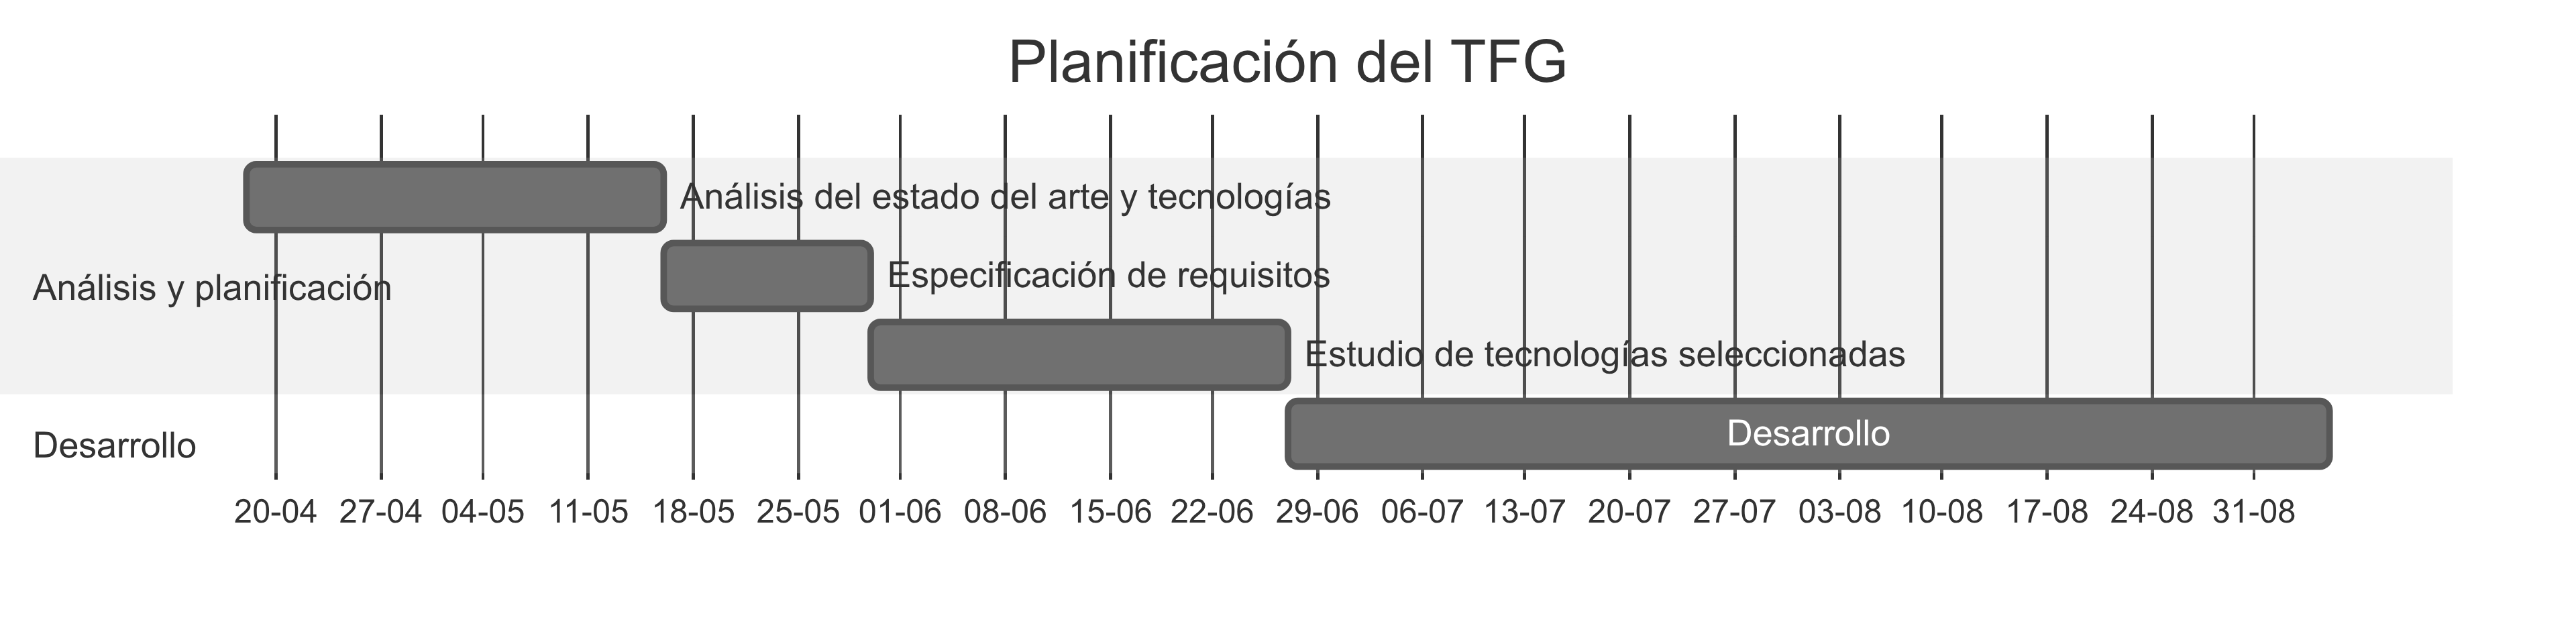
\includegraphics[width=\textwidth]{assets/planificacion-inicial.png}
    \end{center}
    \caption{Diagrama de Gantt de la planificación inicial del proyecto}\label{fig:planificacion-inicial}
\end{figure}


\section{Análisis de costes}
\label{sec:presupuesto}
Para el cálculo y desglose del presupuesto total del proyecto se ha supuesto un equipo de una única persona a media jornada (20 horas semanales).

Para el cálculo del presupuesto de personal hemos tenido en cuenta el salario medio de un ingeniero de software en España, que según el portal de empleo \href{https://www.glassdoor.es/Sueldos/granada-software-engineer-sueldo-SRCH_IL.0,7_IC2614045_KO8,25.htm}{Glassdoor} ronda entre los 24.000 y 33.000 euros brutos anuales, cogiendo el valor de 30.000 euros brutos anuales como salario base dado que se trata de un estudiante en prácticas con conocimientos técnicos avanzados.

Para calcular el costo total mensual de un trabajador, tenemos que sumar al salario base los costes de seguridad social, la cuota patronal, siguiendo la siguiente fórmula:
\begin{equation}
    \text{Coste total mensual} = \text{Salario base} + \text{Seguridad Social} + \text{Cuota patronal}
\end{equation}
\begin{itemize}
    \item Salario base: 30.000 euros brutos anuales / 12 meses / 2 = 1.250 euros brutos mensuales (media jornada)
    \item Seguridad social: 6,45\% sobre el salario bruto mensual:
        \begin{equation}
            \text{Seguridad Social} = 1250 \times 0.0645 = 80.63 \text{ euros mensuales}
        \end{equation}
    \item Cuota patronal: 
        \begin{equation}
            \text{Cuota patronal} = \dfrac{1532.10 \times 0.3198}{2} = 245.12 \text{ euros mensuales}
        \end{equation}
\end{itemize}

De esta manera, el coste total mensual del trabajador sería:
\begin{equation}
    \text{Coste total mensual} = 1250 + 80.63 + 245.12 = 1574.75 \text{ euros mensuales}
\end{equation}

La duración total del proyecto es de aproximadamente 4,67 meses (20 semanas, 400 horas aprox.), por lo que el coste total en personal asciende a:
\begin{equation}
    \text{Coste total personal} = 1574.75 \times 4.67 = 7354.08 \text{ euros}
\end{equation}

Para el gasto de materiales solamente tendremos materiales inventariables, concretamente el material de trabajo del trabajador:
\begin{itemize}
    \item Ordenador de sobremesa: 1.000 euros con vida estimada restante de 4 años, es decir, 250 euros al año.
    \item Monitores: 300 euros con vida estimada restante de 6 años, es decir, 50 euros al año.
    \item Teclado y ratón: 150 euros con vida estimada restante de 3 años, es decir, 50 euros al año.
\end{itemize}
\begin{equation}
    \text{Coste total de materiales} = \dfrac{250 + 50 + 50}{12} \times 4.67 = 146.25 \text{ euros}
\end{equation}

Dado que uno de los objetivos principales del proyecto es la capacidad de alojar la aplicación en un servidor propio previamente ya existente, no tenemos en cuenta el coste de un servidor.

Dado que la aplicación se ha desarrollado usando tecnologías open source, no se han tenido en cuenta los costes de licencias de software.

Se realizará una formación del trabajador antes de comenzar con las fases de planificación y desarrollo. Para la formación del trabajador se han usado cursos gratuitos así como la documentación oficial de las tecnologías utilizadas, por lo que no se ha tenido en cuenta ningún coste adicional.

De esta forma, tendríamos el siguiente desglose de costes:
\begin{table}[H]
    \caption{Tabla de presupuesto del proyecto}\label{tab:presupuesto}
    \begin{center}
        \begin{tabularx}{\textwidth}{|X|c|c|c|}
            \hline
            \textbf{Gastos elegibles} & \textbf{Unidades} & \textbf{Coste por unidad} & \textbf{Importe solicitado} \\
            \hline
            \multicolumn{3}{|l|}{\textbf{GASTOS DE PERSONAL}} & \textbf{7.354,08\euro} \\
            Total gastos de contratación de personal & 4,67 & 1.574,75\euro/mes & 7.354,08\euro \\
            \hline
            \multicolumn{3}{|l|}{\textbf{GASTOS DE EJECUCIÓN}} & \textbf{146,25\euro} \\
            \multicolumn{3}{|l|}{Costes de adquisición de material inventariable} & 146,25\euro \\
            \quad Ordenador & 1 & 97,22\euro & 97,22\euro \\
            \quad Monitores & 1 & 19,45\euro & 19,45\euro \\
            \quad Teclado y ratón & 1 & 29,58\euro & 29,58\euro \\
            \multicolumn{3}{|l|}{Costes de adquisición de material fungible} & 0\euro \\
            \multicolumn{3}{|l|}{Costes de consultoría, prestación de servicios, suministros, etc.} & 0\euro \\
            \multicolumn{3}{|l|}{Costes de subcontratación} & 0\euro \\
            \multicolumn{3}{|l|}{\textbf{GASTOS COMPLEMENTARIOS}} & \textbf{0\euro} \\
            \multicolumn{3}{|l|}{Formación del equipo de desarrollo} & 0\euro \\
            \multicolumn{3}{|l|}{Gastos de desplazamiento, viajes, estancias y dietas} & 0\euro \\
            \multicolumn{3}{|l|}{Gastos de inscripción en congresos y seminarios} & 0\euro \\
            \hline
            \multicolumn{3}{|l|}{\textbf{COSTES DIRECTOS (10\% presupuesto total)}} & \textbf{750,03\euro} \\
            \hline
            \multicolumn{3}{|l|}{\textbf{TOTAL INCENTIVO SOLICITADO}} & \textbf{8.250,363\euro} \\
            \hline
        \end{tabularx}
    \end{center}
\end{table}



\section{Estructura del documento}
Esta memoria se organiza en varios capítulos que abordan de manera progresiva el desarrollo del proyecto, desde su el desarrollo teórico hasta la implementación práctica y sus conclusiones.

En primer lugar, el \textbf{Resumen} y los \textbf{Agradecimientos} ofrecen una visión general y un reconocimiento a quienes han apoyado la realización de este proyecto. A continuación, la \textbf{Introducción} presenta el contexto, la motivación y los objetivos que guían este trabajo, junto con una planificación inicial y un análisis de costes.

El capítulo de \textbf{Estado del Arte} realiza un análisis exhaustivo de las soluciones existentes, tanto propietarias como de código abierto, identificando sus fortalezas, debilidades y las tecnologías que emplean. Este estudio fundamenta las decisiones tomadas y destaca las aportaciones originales de nuestra propuesta.

La sección de \textbf{Análisis de Tecnologías} profundiza en las herramientas y lenguajes de programación considerados para el desarrollo, justificando la elección de Rust para el servidor y Lynx.js para el cliente móvil en base a criterios de rendimiento, seguridad y escalabilidad.

El núcleo de la memoria se encuentra en el capítulo de la \textbf{Propuesta}, donde se detalla la metodología de desarrollo ágil (Scrum) adoptada y se describe la arquitectura del sistema. Este capítulo se complementa con las secciones dedicadas a cada \textbf{Sprint}, en los que se documenta el progreso iterativo del proyecto, detallando las historias de usuario implementadas y las decisiones técnicas tomadas.

Finalmente, las \textbf{Conclusiones y Trabajo Futuro} recogen una reflexión sobre los resultados alcanzados, el cumplimiento de los objetivos, los problemas encontrados y las futuras líneas de trabajo que se abren a partir de este proyecto.
